\documentclass[14pt]{matmex-diploma-custom}

\usepackage[section]{placeins}

\begin{document}

\filltitle{ru}{
	chair              = {Математическое обеспечение и администрирование информационных систем\\Кафедра информационно-аналитических систем},
	title              = {Построение гибридной рекомендательной системы новостей с применением методов оптимизации},
	type               = {diploma},
	position           = {студента},
	group              = 441,
	author             = {Смирнов Александр Львович},
	supervisorPosition = {к.ф.-м.н., доц.},
	supervisor         = {Михайлова Елена Георгиевна}
}

\maketitle

\tableofcontents


\section*{Введение}

Невозможно представить современное приложение, оперирующее большими объёмами информации, без рекомендательной системы. Информации становится настолько много, что пользователи не имеют возможности найти интересный себе контент. Для решения данной проблемы применяются рекомендательные системы.

Рекомендательная система -- совокупность алгоритмов, которые принимают на вход данные об активности пользователей и информацию о рекомендуемых предметах (дата создания, источник и т.д.) и на выходе выдают список предметов, отранжированный по мере того, насколько он релевантен конкретному пользователю.

Компании IT Service требуется рекомендательная система новостей, для того, чтобы увеличить вовлечённость пользователей путём рекомендации релевантного контента.
Ключевым фактором является то, что отстутствует информация о действиях пользователей, вследствие чего не представляется возможным оценить работу алгоритмов на реальных данных.

\section{Постановка задачи}

Целью данной работы является построение и оптимизация гибридной рекомендательной системы новостей. Для её достижения необходимо решить следующие задачи:

\begin{itemize}
	\item провести обзор существующих решений
	\item реализовать каждое уникальное решение и оценить его
	\item соединить различные решения в единую систему
	\item найти оптимальный вклад каждого отдельного решения в результирующий список рекомендаций
\end{itemize}


\section{Обзор}

\subsection{Методы}

В области рекомендательных систем различают два основных подхода:

\begin{itemize}
	\item collaborative filtering
	      \begin{itemize}
		      \item рекомендации на основе действий других пользователей
	      \end{itemize}
	\item content-based filtering
	      \begin{itemize}
		      \item рекомендации на основе содержимого
	      \end{itemize}
\end{itemize}

Оба подхода обладают своими плюсами и минусами. К плюсам коллаборативной фильтрации можно отнести отсутствие необходимости знать что-либо о рекомендуемом предмете, так как рекомендации строятся на основе действий других пользователей. К минусам относится необходимость иметь данные об активности других пользователей, что называется ''холодный старт''.

В свою очередь рекомендации на основе контента не требуют данных о действиях других пользователей, но необходимы признаки, которыми обладает рекомендуемый предмет, для построения вектора предпочтений пользователя.


\subsection{Подходы}

Для коллаборативной фильтрации используют метод kNN \cite{wiki:knn} и корреляцию Пирсона для нахождения похожих векторов.

Для рекомендации на основе содержимого используются байесовский классификатор, решающие деревья, кластерный анализ.

\section{Решение}

В качестве решения предлагается комбинация подходов:

\begin{figure}[h]
	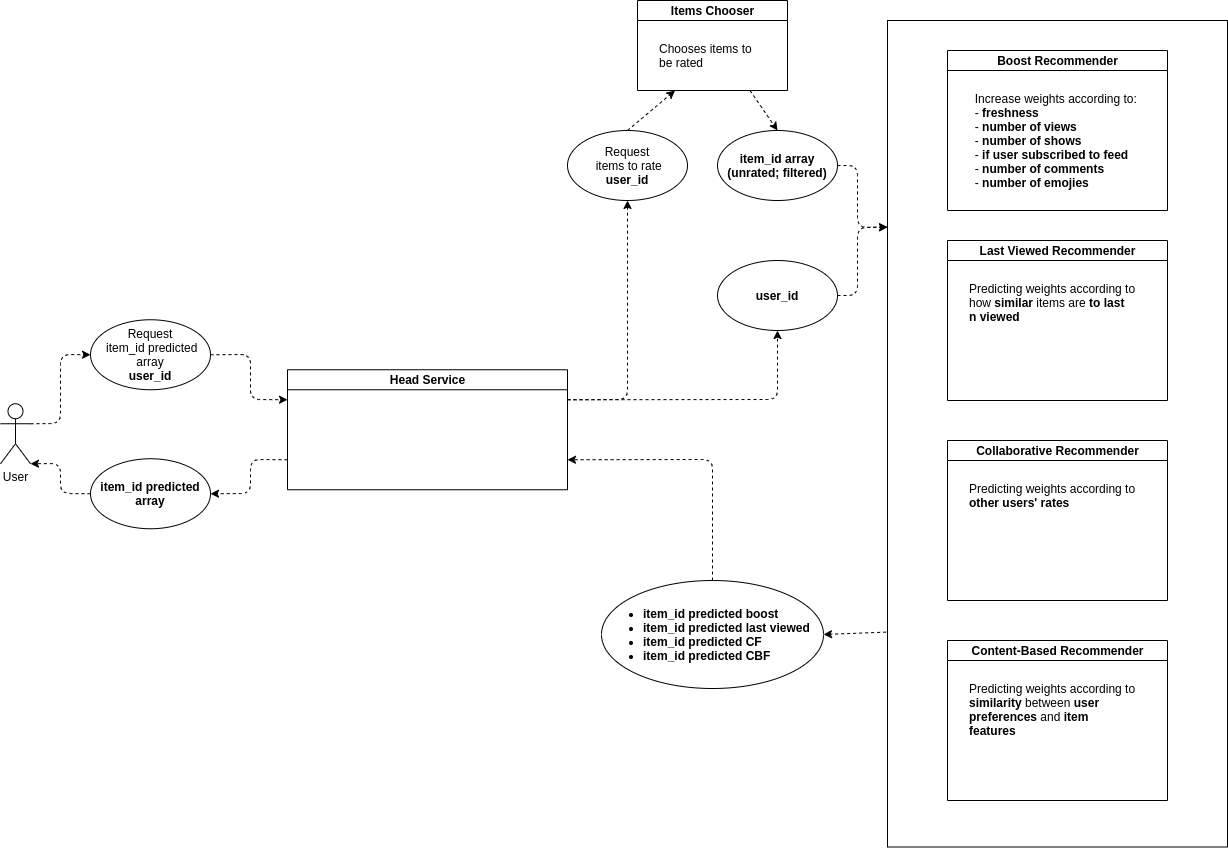
\includegraphics[width=0.9\textwidth]{./images/main.png}
	\centering
\end{figure}

Подходы:

\begin{itemize}
	\item Content-based recommender
	\item Collaborative recommender
	\item Session recommender
	      \begin{itemize}
		      \item рекомендации на основе последних просмотренных элементов
	      \end{itemize}
	\item Boost recommender
	      \begin{itemize}
		      \item рекомендации на основе информации об элементе
	      \end{itemize}
\end{itemize}

Каждый из сервисов уже был реализован, остаётся решить задачу оптимизации, то есть найти подходящие веса для каждого из подходов.

\section{Дальнейшие планы}

В начале января планируется релиз приложение и масштабная пиар-компания, вследствие чего будет доступно очень много логов пользовательской активности.

Собирая и используя эту информацию мы сможем оценить качество построенных моделей.

Также планируется проводить A / B тестирование.


\setmonofont[Mapping=tex-text]{CMU Typewriter Text}
\bibliographystyle{ugost2008ls}
\bibliography{diploma.bib}
\end{document}
